% Campus Marketplace - Technical Architecture & System Design
% Converted from the provided architecture report and extended with:
% 1. Borrow/Lend due-date tracking
% 2. Price-drop alerts
% 3. User Trust Score

\documentclass[11pt,a4paper]{article}

\usepackage[margin=1in]{geometry}
\usepackage[T1]{fontenc}
\usepackage[utf8]{inputenc}
\usepackage{lmodern}
\usepackage{xcolor}
\usepackage{graphicx}
\usepackage{booktabs}
\usepackage{array}
\usepackage{longtable}
\usepackage{tabularx}
\usepackage{enumitem}
\usepackage{float}
\usepackage{tikz}
\usepackage{amsmath}
\usepackage{hyperref}
\usepackage{fancyhdr}
\usepackage{titlesec}
\usepackage{listings}

\usetikzlibrary{arrows.meta,positioning,shapes.geometric,fit,calc}

\definecolor{primary}{RGB}{35,82,180}
\definecolor{secondary}{RGB}{70,70,70}
\definecolor{lightblue}{RGB}{235,242,255}
\definecolor{lightgreen}{RGB}{232,248,239}
\definecolor{lightorange}{RGB}{255,244,225}
\definecolor{lightred}{RGB}{255,235,235}

\hypersetup{
    colorlinks=true,
    linkcolor=primary,
    urlcolor=primary,
    citecolor=primary,
    pdftitle={Campus Marketplace - Technical Architecture and System Design}
}

\pagestyle{fancy}
\fancyhf{}
\lhead{\textit{Campus Marketplace}}
\rhead{\textit{Technical Architecture}}
\cfoot{\thepage}

\titleformat{\section}
  {\Large\bfseries\color{primary}}
  {\thesection.}{0.5em}{}
\titleformat{\subsection}
  {\large\bfseries\color{primary}}
  {\thesubsection}{0.5em}{}

\setlist[itemize]{noitemsep,topsep=3pt}
\setlist[enumerate]{noitemsep,topsep=3pt}

\newcolumntype{Y}{>{\raggedright\arraybackslash}X}
\newcolumntype{P}[1]{>{\raggedright\arraybackslash}p{#1}}

\tikzset{
    box/.style={draw=primary, rounded corners, thick, fill=lightblue,
        minimum height=0.75cm, minimum width=2.3cm, align=center},
    greenbox/.style={draw=green!50!black, rounded corners, thick, fill=lightgreen,
        minimum height=0.75cm, minimum width=2.3cm, align=center},
    orangebox/.style={draw=orange!70!black, rounded corners, thick, fill=lightorange,
        minimum height=0.75cm, minimum width=2.3cm, align=center},
    redbox/.style={draw=red!60!black, rounded corners, thick, fill=lightred,
        minimum height=0.75cm, minimum width=2.3cm, align=center},
    arrow/.style={-{Latex[length=2mm]}, thick, draw=secondary}
}

\begin{document}

\begin{titlepage}
    \centering
    \vspace*{2cm}
    {\Huge\bfseries\color{primary} TECHNICAL ARCHITECTURE\\[0.2cm]
    \& SYSTEM DESIGN\par}
    \vspace{1cm}
    {\LARGE\bfseries Campus Marketplace\par}
    \vspace{0.5cm}
    {\Large AI Pricing \& Fraud Detection for a Verified Student Trading Ecosystem\par}
    \vspace{1.2cm}

    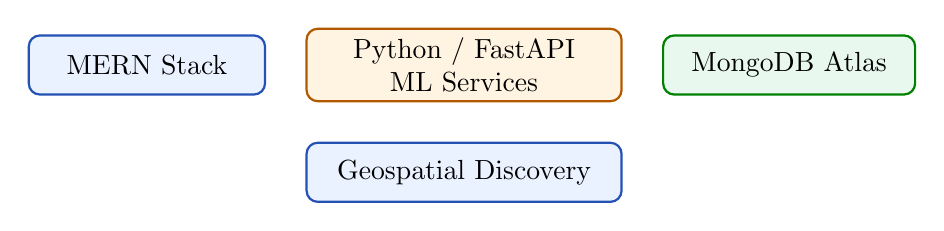
\begin{tikzpicture}
        \node[box, minimum width=3cm] (mern) {MERN Stack};
        \node[orangebox, right=0.5cm of mern, minimum width=4cm] (ml)
            {Python / FastAPI\\ML Services};
        \node[greenbox, right=0.5cm of ml, minimum width=3.2cm] (db)
            {MongoDB Atlas};
        \node[box, below=0.5cm of ml, minimum width=4cm] (geo)
            {Geospatial Discovery};
    \end{tikzpicture}

    \vfill
    {\large Academic Project Proposal\\August 2026\par}
\end{titlepage}

\tableofcontents
\newpage

\section{What We Are Building \& Why}

Campus Marketplace is a campus-exclusive platform where verified students buy, sell, lend, and borrow used items such as textbooks, cycles, electronics, lab gear, furniture, notes, and hostel items.

It differs from a generic classifieds application in three ways:
\begin{enumerate}
    \item Access is restricted to verified institutional email holders.
    \item An AI pricing engine tells buyers and sellers whether an asking price is fair.
    \item A fraud-risk model screens listings and accounts before problems reach students.
\end{enumerate}

The extended system additionally provides:
\begin{itemize}
    \item \textbf{Borrow/Lend Due-Date Tracking} for temporary item transactions.
    \item \textbf{Price-Drop Alerts} for buyers watching an item.
    \item \textbf{Trust Score} based on verified activity, transaction history, reviews, and reports.
\end{itemize}

The goal is a safe, transparent, AI-assisted trading ecosystem---not a full e-commerce clone.

\begin{figure}[H]
\centering
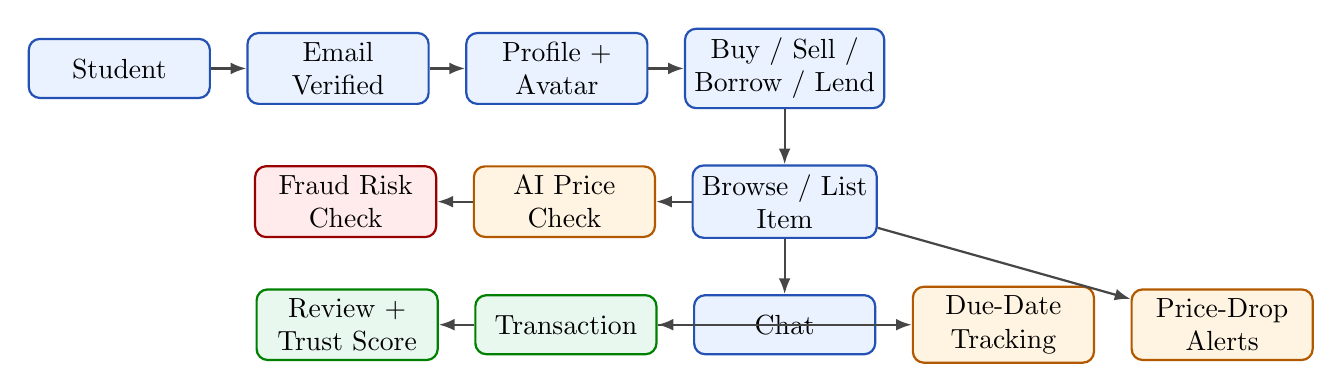
\begin{tikzpicture}[node distance=0.7cm and 0.45cm]
\node[box] (student) {Student};
\node[box, right=of student] (verify) {Email\\Verified};
\node[box, right=of verify] (profile) {Profile +\\Avatar};
\node[box, right=of profile] (action) {Buy / Sell /\\Borrow / Lend};
\node[box, below=of action] (browse) {Browse / List\\Item};
\node[orangebox, left=of browse] (price) {AI Price\\Check};
\node[redbox, left=of price] (fraud) {Fraud Risk\\Check};
\node[box, below=of browse] (chat) {Chat};
\node[greenbox, left=of chat] (transaction) {Transaction};
\node[greenbox, left=of transaction] (review) {Review +\\Trust Score};
\node[orangebox, right=of chat] (due) {Due-Date\\Tracking};
\node[orangebox, right=of due] (alert) {Price-Drop\\Alerts};

\draw[arrow] (student)--(verify);
\draw[arrow] (verify)--(profile);
\draw[arrow] (profile)--(action);
\draw[arrow] (action)--(browse);
\draw[arrow] (browse)--(price);
\draw[arrow] (price)--(fraud);
\draw[arrow] (browse)--(chat);
\draw[arrow] (chat)--(transaction);
\draw[arrow] (transaction)--(review);
\draw[arrow] (transaction)--(due);
\draw[arrow] (browse)--(alert);
\end{tikzpicture}
\caption{High-level end-to-end system flow. AI pricing and fraud checks run in parallel with normal marketplace activity.}
\end{figure}

\section{User Roles}

Students are not locked into a fixed role. After login, they choose an action from the dashboard.

\begin{table}[H]
\centering
\begin{tabularx}{\textwidth}{P{0.23\textwidth}Y}
\toprule
\textbf{Role} & \textbf{Capabilities}\\
\midrule
Student & Buy, sell, borrow, lend, browse, chat, transact, review users, watch listings, receive price-drop alerts.\\
Borrower & Request borrowed items, accept terms, view due dates, receive return reminders, mark items returned.\\
Lender & List items for lending, set lending duration/due date, approve borrowers, track active and overdue loans.\\
Admin & Institution configuration, monitor listings, review fraud alerts, handle reports, suspend users, remove listings, analytics, and banned-word/category management.\\
\bottomrule
\end{tabularx}
\end{table}

\section{College Email Verification}

\begin{center}
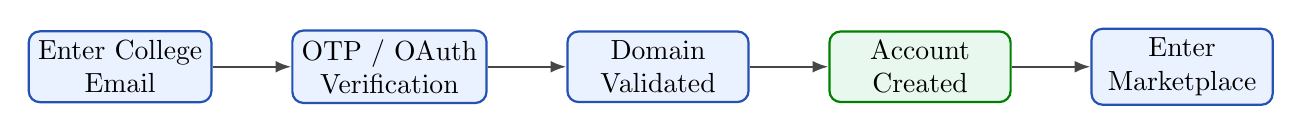
\begin{tikzpicture}[node distance=1cm]
\node[box] (email) {Enter College\\Email};
\node[box, right=of email] (otp) {OTP / OAuth\\Verification};
\node[box, right=of otp] (domain) {Domain\\Validated};
\node[greenbox, right=of domain] (account) {Account\\Created};
\node[box, right=of account] (market) {Enter\\Marketplace};
\draw[arrow] (email)--(otp);
\draw[arrow] (otp)--(domain);
\draw[arrow] (domain)--(account);
\draw[arrow] (account)--(market);
\end{tikzpicture}
\end{center}

Domain matching confirms institutional affiliation only, not trustworthiness. Email verification is therefore combined with CAPTCHA/rate limiting, duplicate-account detection, report/block tools, and admin moderation.

\subsection{Avatar-Based Identity}

Users build an identity from predefined components such as face, hair, clothing, accessories, and colour. These are stored as a small JSON object in the \texttt{Users} collection. Real photos are not required, reducing onboarding friction and the safety/moderation burden.

AI-generated avatars are left as a future enhancement.

\section{Optional Location-Based Discovery}

Location sharing is off by default and fully opt-in. Exact coordinates are never shown publicly. Only approximate/geohashed positions are used for discovery, while precise meeting points are revealed only after both parties agree.

\begin{center}
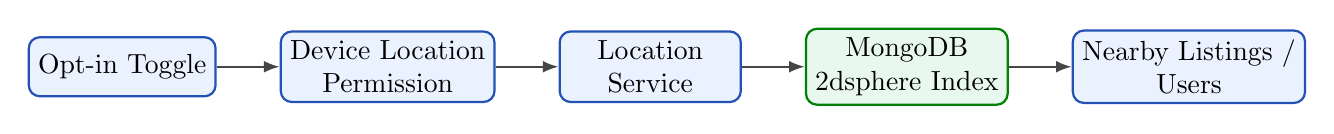
\begin{tikzpicture}[node distance=0.8cm]
\node[box] (toggle) {Opt-in Toggle};
\node[box, right=of toggle] (permission) {Device Location\\Permission};
\node[box, right=of permission] (service) {Location\\Service};
\node[greenbox, right=of service] (mongo) {MongoDB\\2dsphere Index};
\node[box, right=of mongo] (nearby) {Nearby Listings /\\Users};
\draw[arrow] (toggle)--(permission);
\draw[arrow] (permission)--(service);
\draw[arrow] (service)--(mongo);
\draw[arrow] (mongo)--(nearby);
\end{tikzpicture}
\end{center}

MongoDB's \texttt{\$geoNear}/\texttt{\$near} queries support nearby searches directly on a geospatial index.

\textbf{Safeguards:}
\begin{itemize}
    \item Disable location sharing at any time.
    \item Never publish exact coordinates.
    \item Use geohash rounding for approximate discovery.
    \item Reveal precise location only after mutual agreement.
    \item Encrypt stored location data.
    \item Automatically expire stale location data.
\end{itemize}

\section{AI Price Recommendation}

Rather than returning a single number, the model returns a fair price range, confidence score, and plain-language reason. This helps both sellers and buyers assess whether an asking price is reasonable.

\begin{center}
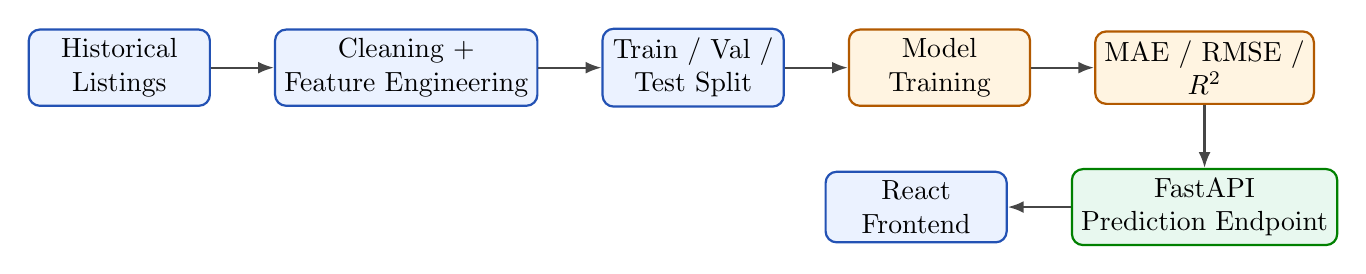
\begin{tikzpicture}[node distance=0.8cm]
\node[box] (data) {Historical\\Listings};
\node[box, right=of data] (clean) {Cleaning +\\Feature Engineering};
\node[box, right=of clean] (split) {Train / Val /\\Test Split};
\node[orangebox, right=of split] (train) {Model\\Training};
\node[orangebox, right=of train] (eval) {MAE / RMSE /\\$R^2$};
\node[greenbox, below=0.8cm of eval] (api) {FastAPI\\Prediction Endpoint};
\node[box, left=of api] (front) {React\\Frontend};
\draw[arrow] (data)--(clean);
\draw[arrow] (clean)--(split);
\draw[arrow] (split)--(train);
\draw[arrow] (train)--(eval);
\draw[arrow] (eval)--(api);
\draw[arrow] (api)--(front);
\end{tikzpicture}
\end{center}

\textbf{Features:} original price, age, condition, brand, category, demand, and prior campus listings.

\begin{table}[H]
\centering
\begin{tabularx}{\textwidth}{P{0.28\textwidth}Y}
\toprule
\textbf{Model} & \textbf{Recommendation}\\
\midrule
Linear Regression & Good simple baseline; may struggle with nonlinear condition and brand effects.\\
Random Forest Regressor & Recommended for v1; handles mixed numeric/categorical features well and is robust on a small campus dataset.\\
Gradient Boosting / XGBoost & Potential v2 upgrade once more labelled data accumulates.\\
\bottomrule
\end{tabularx}
\end{table}

Accuracy is intentionally not overclaimed: outputs are framed as an ``AI-estimated fair range'', not a guaranteed price.

\section{Fraud / Scam Detection}

Detection operates at three levels:
\begin{itemize}
    \item \textbf{Listing:} price outliers, reused images, duplicate posts.
    \item \textbf{User:} multiple accounts, rapid listing bursts, prior reports.
    \item \textbf{Behavioural:} unusual activity spikes.
\end{itemize}

The system produces a single \textbf{Fraud Risk Score} that flags suspicious activity rather than automatically accusing a user.

\begin{center}
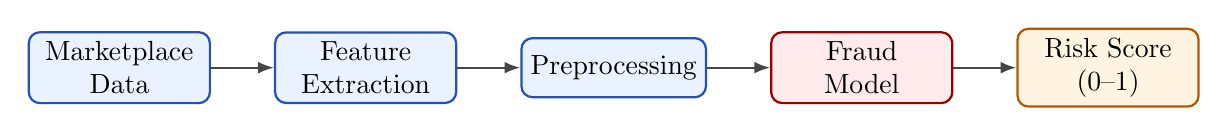
\begin{tikzpicture}[node distance=0.8cm]
\node[box] (data) {Marketplace\\Data};
\node[box, right=of data] (features) {Feature\\Extraction};
\node[box, right=of features] (prep) {Preprocessing};
\node[redbox, right=of prep] (model) {Fraud\\Model};
\node[orangebox, right=of model] (score) {Risk Score\\(0--1)};
\draw[arrow] (data)--(features);
\draw[arrow] (features)--(prep);
\draw[arrow] (prep)--(model);
\draw[arrow] (model)--(score);
\end{tikzpicture}
\end{center}

\begin{center}
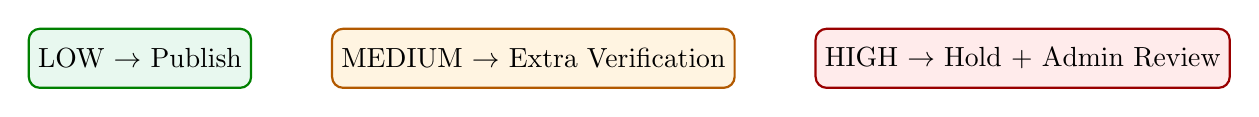
\begin{tikzpicture}[node distance=0.9cm]
\node[greenbox] (low) {LOW $\rightarrow$ Publish};
\node[orangebox, right=1cm of low] (medium) {MEDIUM $\rightarrow$ Extra Verification};
\node[redbox, right=1cm of medium] (high) {HIGH $\rightarrow$ Hold + Admin Review};
\end{tikzpicture}
\end{center}

The recommended initial approach is Isolation Forest (unsupervised anomaly detection), since labelled fraud data will not exist initially. Logistic Regression or Random Forest can be introduced later when sufficient confirmed-fraud labels are collected from admin reviews.

\section{Combined AI Decision Engine}

\begin{center}
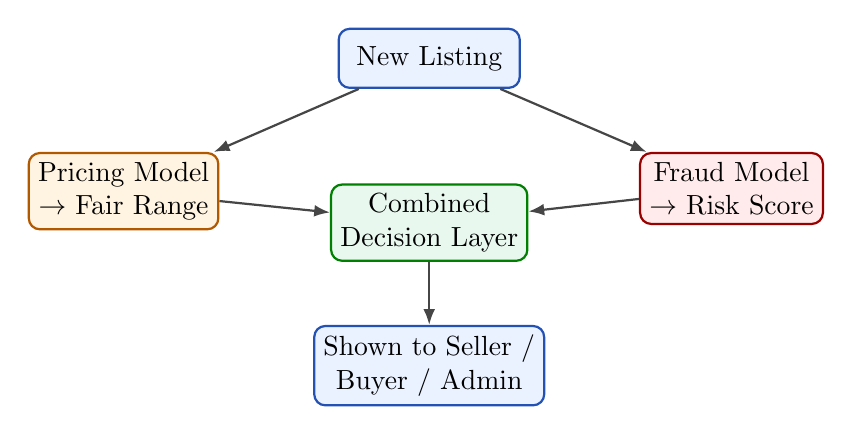
\begin{tikzpicture}[node distance=0.8cm and 1.5cm]
\node[box] (listing) {New Listing};
\node[orangebox, below left=of listing] (pricing) {Pricing Model\\$\rightarrow$ Fair Range};
\node[redbox, below right=of listing] (fraud) {Fraud Model\\$\rightarrow$ Risk Score};
\node[greenbox, below=1.2cm of listing] (combined) {Combined\\Decision Layer};
\node[box, below=of combined] (shown) {Shown to Seller /\\Buyer / Admin};

\draw[arrow] (listing)--(pricing);
\draw[arrow] (listing)--(fraud);
\draw[arrow] (pricing)--(combined);
\draw[arrow] (fraud)--(combined);
\draw[arrow] (combined)--(shown);
\end{tikzpicture}
\end{center}

For example, an iPhone 13 listed 30\% below the estimated market range does not automatically become a fraud case. Price deviation is only one signal among several weighted by the risk model.

\section{Borrow/Lend Due-Date Tracking}

Borrowing and lending are treated as first-class transaction types rather than simple sales.

\subsection{Borrow/Lend Workflow}

\begin{center}
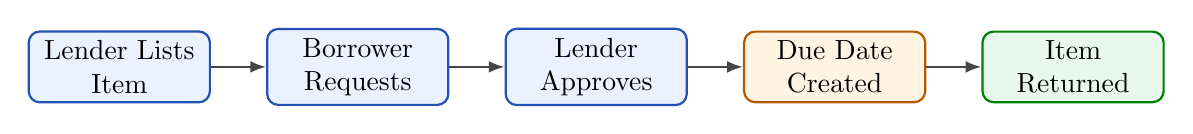
\begin{tikzpicture}[node distance=0.7cm]
\node[box] (list) {Lender Lists\\Item};
\node[box, right=of list] (request) {Borrower\\Requests};
\node[box, right=of request] (approve) {Lender\\Approves};
\node[orangebox, right=of approve] (due) {Due Date\\Created};
\node[greenbox, right=of due] (return) {Item\\Returned};
\draw[arrow] (list)--(request);
\draw[arrow] (request)--(approve);
\draw[arrow] (approve)--(due);
\draw[arrow] (due)--(return);
\end{tikzpicture}
\end{center}

When a lender approves a borrow request, the transaction stores:
\begin{itemize}
    \item Borrower and lender IDs.
    \item Start date.
    \item Due date.
    \item Optional extension count and extension history.
    \item Return status.
    \item Overdue status.
\end{itemize}

The dashboard displays active loans and their remaining time. Automated reminders can be generated before the due date and when an item becomes overdue.

\subsection{Due-Date States}

\begin{center}
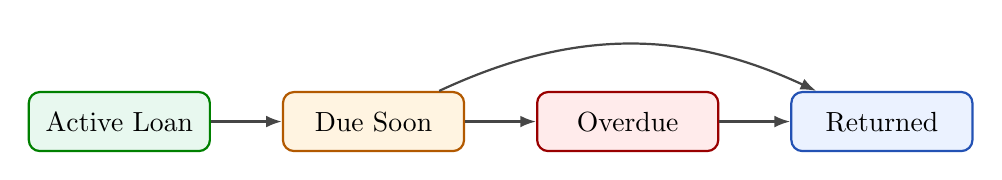
\begin{tikzpicture}[node distance=0.9cm]
\node[greenbox] (active) {Active Loan};
\node[orangebox, right=of active] (soon) {Due Soon};
\node[redbox, right=of soon] (overdue) {Overdue};
\node[box, right=of overdue] (returned) {Returned};
\draw[arrow] (active)--(soon);
\draw[arrow] (soon)--(overdue);
\draw[arrow] (overdue)--(returned);
\draw[arrow] (soon) to[bend left=25] (returned);
\end{tikzpicture}
\end{center}

\textbf{Business rules:}
\begin{itemize}
    \item A due date is mandatory for borrow/lend transactions.
    \item Borrowers receive a reminder before the due date.
    \item Overdue transactions are visible to both parties and the admin system.
    \item Repeated overdue returns can reduce a user's Trust Score.
    \item A lender may accept or reject an extension request.
    \item A transaction can be marked complete only after the lender confirms return.
\end{itemize}

\section{Price-Drop Alerts}

Users can save/watch a listing and choose to receive an alert when its price decreases.

\subsection{Alert Logic}

\begin{center}
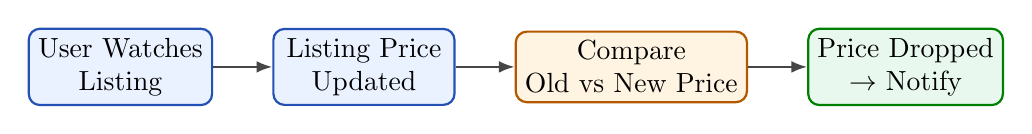
\begin{tikzpicture}[node distance=0.75cm]
\node[box] (watch) {User Watches\\Listing};
\node[box, right=of watch] (price) {Listing Price\\Updated};
\node[orangebox, right=of price] (compare) {Compare\\Old vs New Price};
\node[greenbox, right=of compare] (alert) {Price Dropped\\$\rightarrow$ Notify};
\draw[arrow] (watch)--(price);
\draw[arrow] (price)--(compare);
\draw[arrow] (compare)--(alert);
\end{tikzpicture}
\end{center}

The alert service stores the user's watch preferences and the last observed price. When the seller lowers the listed price, the system generates an in-app notification and can optionally send an email notification.

A basic rule is:
\[
\text{Price Drop} =
\begin{cases}
1, & P_{\mathrm{new}} < P_{\mathrm{old}}\\
0, & \text{otherwise}
\end{cases}
\]

Optional future refinement can trigger alerts only when the reduction exceeds a user-selected threshold such as 5\% or a fixed amount.

\section{Trust Score}

The \textbf{Trust Score} provides a compact representation of a user's marketplace reliability. It is not the same as the AI Fraud Risk Score: fraud risk evaluates suspicious behaviour, whereas Trust Score represents accumulated positive and negative transaction history.

\subsection{Trust Score Inputs}

The score can consider:
\begin{itemize}
    \item Verified institutional account.
    \item Successful completed transactions.
    \item Average review rating.
    \item Number of positive reviews.
    \item On-time return rate for borrowed items.
    \item Number and severity of confirmed reports.
    \item Overdue borrow/lend history.
    \item Account age and normal marketplace activity.
\end{itemize}

A simple normalized formulation for the initial implementation is:
\[
T = w_vV + w_rR + w_cC + w_oO - w_fF
\]
where:
\begin{itemize}
    \item $V$ = verification component,
    \item $R$ = review/rating component,
    \item $C$ = completed transaction component,
    \item $O$ = on-time return component,
    \item $F$ = confirmed negative-report component,
    \item $w_i$ = configurable weights.
\end{itemize}

The final score is normalized to a 0--100 range.

\begin{table}[H]
\centering
\begin{tabularx}{\textwidth}{P{0.22\textwidth}Y}
\toprule
\textbf{Score Range} & \textbf{Interpretation}\\
\midrule
80--100 & Highly trusted marketplace history\\
60--79 & Good / established history\\
40--59 & Limited or mixed history\\
0--39 & Low trust; additional caution or verification may be appropriate\\
\bottomrule
\end{tabularx}
\end{table}

The score should be presented as a decision-support indicator rather than a guarantee of user behaviour. Confirmed reports should affect the score more strongly than unverified complaints.

\section{Backend Architecture}

A modular monolithic Node.js/Express backend with logically separated modules, plus independent Python/FastAPI ML services, is recommended over full microservices. This is simpler to build, test, and deploy for a project of this scope while keeping AI logic decoupled.

\begin{center}
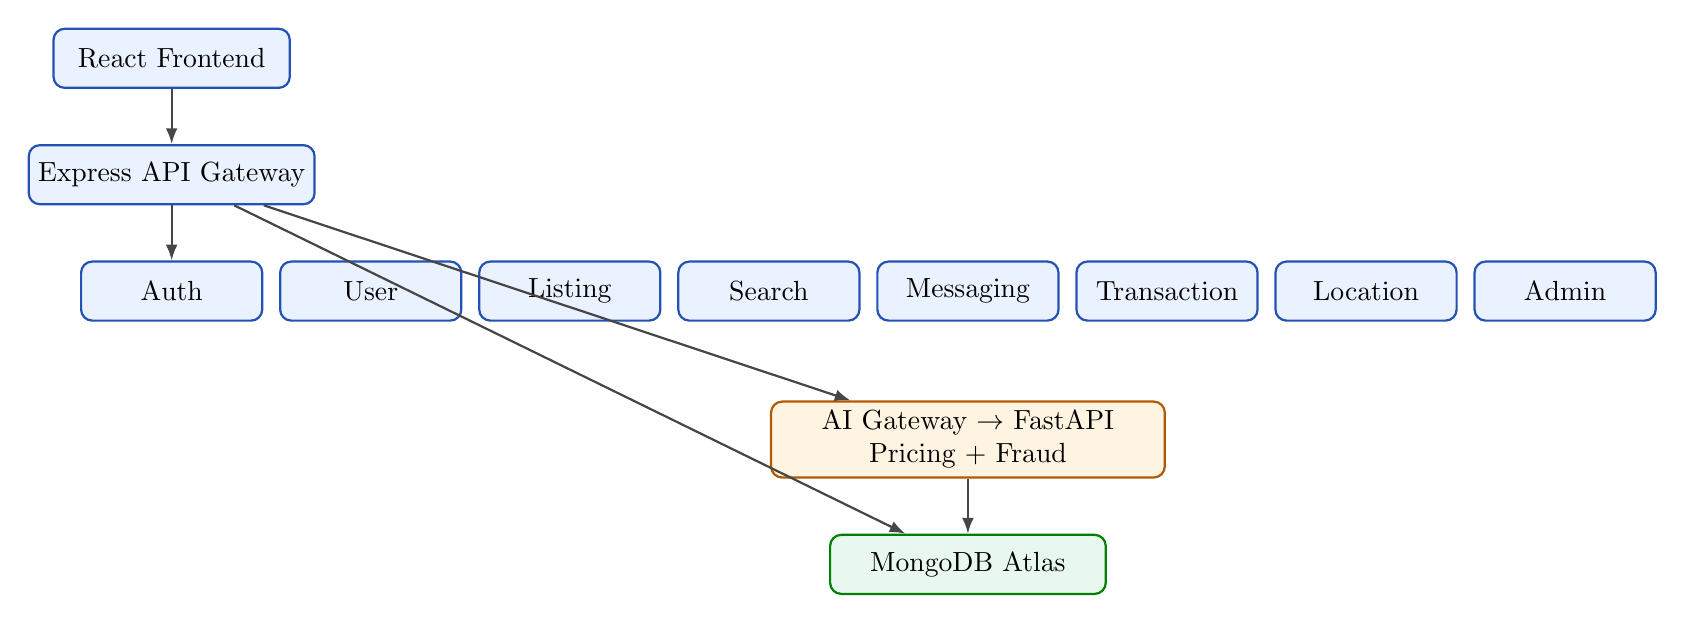
\begin{tikzpicture}[node distance=0.7cm]
\node[box, minimum width=3cm] (react) {React Frontend};
\node[box, below=of react, minimum width=3cm] (express) {Express API Gateway};
\node[box, below=of express] (auth) {Auth};
\node[box, right=0.2cm of auth] (user) {User};
\node[box, right=0.2cm of user] (listing) {Listing};
\node[box, right=0.2cm of listing] (search) {Search};
\node[box, right=0.2cm of search] (message) {Messaging};
\node[box, right=0.2cm of message] (transaction) {Transaction};
\node[box, right=0.2cm of transaction] (location) {Location};
\node[box, right=0.2cm of location] (admin) {Admin};
\node[orangebox, below=1cm of message, minimum width=5cm] (ai)
    {AI Gateway $\rightarrow$ FastAPI\\Pricing + Fraud};
\node[greenbox, below=of ai, minimum width=3.5cm] (mongo) {MongoDB Atlas};

\draw[arrow] (react)--(express);
\draw[arrow] (express)--(auth);
\draw[arrow] (express)--(ai);
\draw[arrow] (ai)--(mongo);
\draw[arrow] (express)--(mongo);
\end{tikzpicture}
\end{center}

\section{Database Schema (MongoDB)}

\begin{longtable}{P{0.19\textwidth}P{0.72\textwidth}}
\toprule
\textbf{Collection} & \textbf{Key Fields}\\
\midrule
\endhead
Users &
userId, collegeEmail, avatar, role/preferences, verificationStatus, trustScore, locationSharingEnabled, approximateLocation, createdAt\\
\addlinespace
Listings &
listingId, sellerId, title, category, condition, images, listedPrice, AIRecommendedPrice, fairPriceRange, fraudRiskScore, listingType (sale/borrow/lend), location, alertEligible\\
\addlinespace
Transactions &
transactionId, buyerId/borrowerId, sellerId/lenderId, listingId, type, status, startDate, dueDate, returnedAt, extensionCount, overdueStatus, createdAt, completedAt\\
\addlinespace
Messages &
messageId, senderId, receiverId, listingId, message, timestamp\\
\addlinespace
Reviews &
reviewerId, reviewedUserId, transactionId, rating, comment\\
\addlinespace
FraudReports &
reportId, reporterId, reportedUserId/listingId, reason, riskScore, status\\
\addlinespace
Watchlists &
watchId, userId, listingId, lastObservedPrice, alertEnabled, thresholdType, thresholdValue, createdAt\\
\addlinespace
Notifications &
notificationId, userId, type, listingId/transactionId, message, readStatus, createdAt\\
\bottomrule
\end{longtable}

\texttt{Listings.location} uses a GeoJSON Point with a 2dsphere index to support nearby-item queries directly in MongoDB.

\section{Key APIs}

\begin{longtable}{P{0.18\textwidth}P{0.72\textwidth}}
\toprule
\textbf{Domain} & \textbf{Endpoints}\\
\midrule
\endhead
Auth & POST \texttt{/auth/register}, \texttt{/verify}, \texttt{/login}, \texttt{/logout}\\
Listings & POST/GET/PUT/DELETE \texttt{/listings[/:id]}\\
AI & POST \texttt{/ai/price-predict}, POST \texttt{/ai/fraud-score}\\
Location & PUT \texttt{/location/preferences}, PUT \texttt{/location}, GET \texttt{/location/nearby}\\
Messages & POST \texttt{/messages}, GET \texttt{/messages/:conversationId}\\
Transactions & POST \texttt{/transactions}, PUT \texttt{/transactions/:id/due-date}, PUT \texttt{/transactions/:id/return}, POST \texttt{/transactions/:id/extend}\\
Watchlist & POST \texttt{/watchlist}, DELETE \texttt{/watchlist/:listingId}, GET \texttt{/watchlist}\\
Alerts & GET \texttt{/notifications}, PUT \texttt{/notifications/:id/read}\\
Trust & GET \texttt{/users/:id/trust-score}\\
Admin & GET \texttt{/admin/fraud-alerts}, PUT \texttt{/admin/listings/:id/review}\\
\bottomrule
\end{longtable}

\section{Security}

\begin{itemize}
    \item College email verification.
    \item Hashed passwords and JWT sessions.
    \item HTTPS.
    \item Input validation and rate limiting.
    \item CORS configuration.
    \item Role-based access control.
    \item Signed image uploads with size/type checks.
    \item Duplicate-account detection.
    \item Geohashed location storage; exact location is never public by default.
    \item Chat abuse reporting.
    \item Admin-only authenticated routes.
    \item Audit trail for trust-score-impacting actions.
\end{itemize}

\section{Deployment Architecture}

\begin{center}
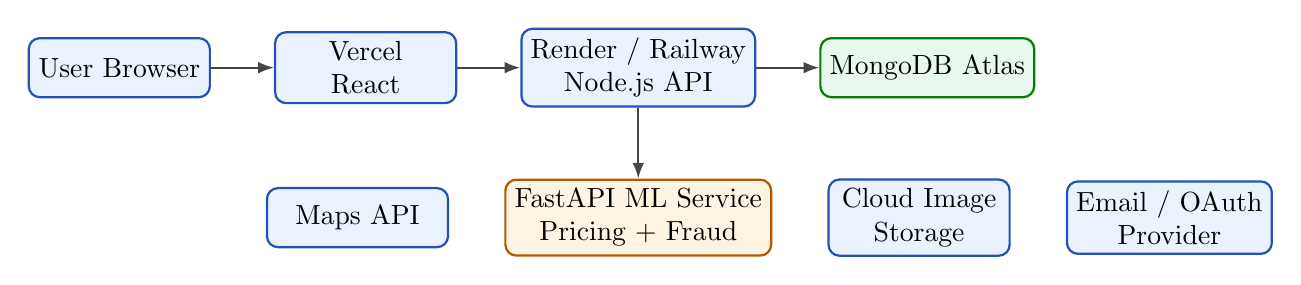
\begin{tikzpicture}[node distance=0.8cm]
\node[box] (browser) {User Browser};
\node[box, right=of browser] (vercel) {Vercel\\React};
\node[box, right=of vercel] (render) {Render / Railway\\Node.js API};
\node[greenbox, right=of render] (mongo) {MongoDB Atlas};
\node[orangebox, below=0.9cm of render] (fastapi) {FastAPI ML Service\\Pricing + Fraud};
\node[box, left=0.7cm of fastapi] (maps) {Maps API};
\node[box, right=0.7cm of fastapi] (storage) {Cloud Image\\Storage};
\node[box, right=0.7cm of storage] (email) {Email / OAuth\\Provider};

\draw[arrow] (browser)--(vercel);
\draw[arrow] (vercel)--(render);
\draw[arrow] (render)--(mongo);
\draw[arrow] (render)--(fastapi);
\end{tikzpicture}
\end{center}

A practical cost-realistic deployment uses managed platforms for the frontend, backend, database, and independently deployed ML service.

Mapbox is recommended for a flexible campus map and a student-friendly deployment model.

\section{MVP vs. Future Enhancements}

\begin{table}[H]
\centering
\begin{tabularx}{\textwidth}{Y P{0.17\textwidth}}
\toprule
\textbf{Feature} & \textbf{Status}\\
\midrule
Email authentication, profiles, avatars, listings, search, messaging, reviews & MVP\\
AI price recommendation using Random Forest & MVP\\
Basic fraud scoring using Isolation Forest & MVP\\
Optional approximate location + admin moderation & MVP\\
Borrow/Lend due-date tracking and overdue reminders & MVP\\
Price-drop alerts and listing watchlist & MVP\\
User Trust Score & MVP\\
Mobile app & Future\\
Computer-vision fraud detection & Future\\
OCR invoices & Future\\
AI chat assistant & Future\\
Escrow/payments & Future\\
Demand forecasting & Future\\
\bottomrule
\end{tabularx}
\end{table}

\section{Final System Pipeline}

\begin{center}
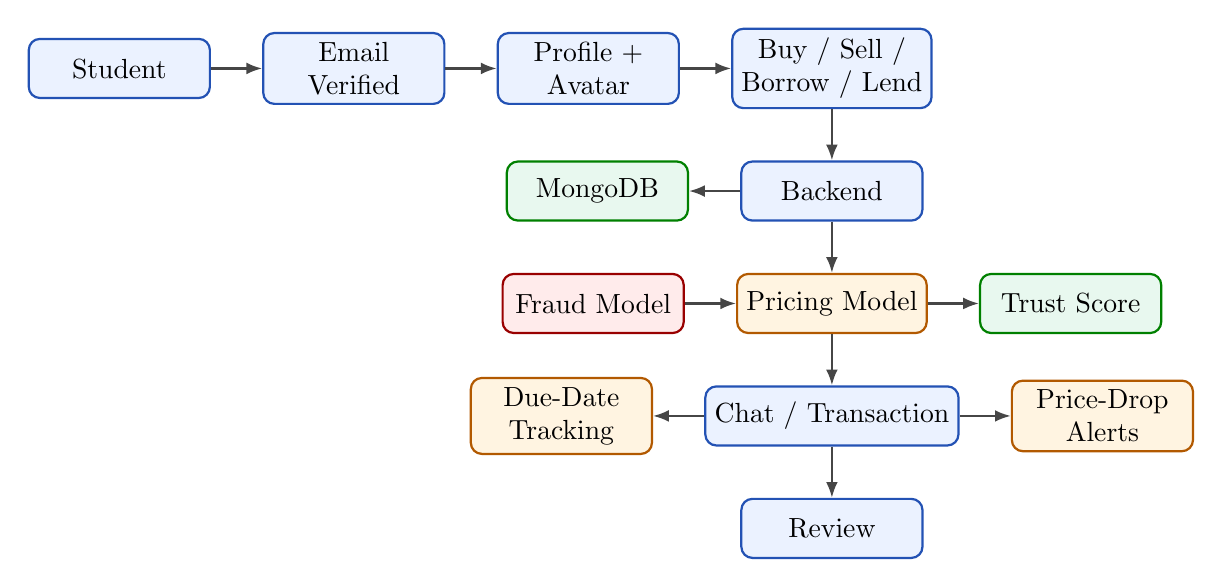
\begin{tikzpicture}[node distance=0.65cm]
\node[box] (student) {Student};
\node[box, right=of student] (verified) {Email\\Verified};
\node[box, right=of verified] (profile) {Profile +\\Avatar};
\node[box, right=of profile] (actions) {Buy / Sell /\\Borrow / Lend};
\node[box, below=of actions] (backend) {Backend};
\node[greenbox, left=of backend] (mongo) {MongoDB};
\node[orangebox, below=of backend] (pricing) {Pricing Model};
\node[redbox, left=of pricing] (fraud) {Fraud Model};
\node[greenbox, right=of pricing] (trust) {Trust Score};
\node[box, below=of pricing] (chat) {Chat / Transaction};
\node[orangebox, left=of chat] (due) {Due-Date\\Tracking};
\node[orangebox, right=of chat] (alerts) {Price-Drop\\Alerts};
\node[box, below=of chat] (review) {Review};
\draw[arrow] (student)--(verified);
\draw[arrow] (verified)--(profile);
\draw[arrow] (profile)--(actions);
\draw[arrow] (actions)--(backend);
\draw[arrow] (backend)--(mongo);
\draw[arrow] (backend)--(pricing);
\draw[arrow] (pricing)--(chat);
\draw[arrow] (fraud)--(pricing);
\draw[arrow] (pricing)--(trust);
\draw[arrow] (chat)--(review);
\draw[arrow] (chat)--(due);
\draw[arrow] (chat)--(alerts);
\end{tikzpicture}
\end{center}

The complete pipeline combines verified student access, marketplace functionality, AI-assisted price estimation, fraud risk scoring, optional geospatial discovery, due-date tracking, price-drop notifications, and trust mechanisms.

\section{Summary}

Campus Marketplace combines a verified campus community, marketplace functionality, AI-assisted price estimation, fraud risk scoring, optional location-based discovery, and trust mechanisms into one ecosystem.

The added features make the platform more useful beyond simple buying and selling:
\begin{itemize}
    \item \textbf{Borrow/Lend Due-Date Tracking} makes temporary transactions manageable and reduces missed returns.
    \item \textbf{Price-Drop Alerts} help buyers discover when a watched item becomes cheaper.
    \item \textbf{Trust Score} gives students a quick view of accumulated marketplace reliability.
\end{itemize}

The AI layer estimates and flags; it does not guarantee fair pricing or eliminate fraud outright. Final decisions on flagged listings remain with admin review.

\begin{center}
\textbf{Campus Marketplace --- Technical Architecture Document}\\
Prepared as an academic project proposal --- August 2026
\end{center}

\end{document}
